Már a legegyszerűbb felhasználói felület láttán is könnyen belátható, hogy a korábbi példaprogramjaink kissé sántítanak, mégpedig abban a tekintetben, hogy nincs olyan valós életben is használt program amiben egy-egy \textit{widget} lenne csupán. Ha viszont több \textit{widget}et szeretnénk elhelyezni egy ablakban kézenfekvő kérdés, hogy miként tudnák őket a felületen csoportokba rendezni. Erre a kérdésre keressük a választ ebben a részben.

\section{Fogalmak}

A korábbiakhoz hasonlóan itt is érdemes először tisztázni néhány alapfogalmat és csak utána kezdeni bele az érdemi munkába.

\subsection{Konténerek}
\index{konténer}

A \textit{widget}ek a felületen történő csoportokba csoportokba rendezése konténerek (\textit{container}) segítségével valósul meg. Ezek olyan láthatatlan \textit{widget}ek, melyekbe más \textit{widget}eket helyezhetünk (\textit{pack}).

\index{GtkContainer@\texttt{GtkContainer}}
A \texttt{GtkContainer} egy önmagában nem használható absztrakt osztály, ami csupán ősül szolgál minden olyan származtatott osztálynak, melyet widgetek tárolására lehet használni.

\index{GtkBin@\texttt{GtkBin}}
\index{GtkBox@\texttt{GtkBox}}
Alapvetően két olyan ősosztállyal találkozhatunk a későbbiekben, melyek további származtatás alapjául szolgálnak. Ezek a \texttt{GtkBin} és a \texttt{GtkBox}. A \texttt{GtkBin} ráadásul absztrakt osztály, azaz csak további származtatás céljára használható, példányosítani nem lehet. Bár a \texttt{GtkBin} és a \texttt{GtkBox} osztályok csupán a bennük tárolható elemek számosságában különböznek egymástól, szerepük mégis gyökeresen eltérő. Előbbi mindössze egy elem tárolására alkalmas, vagyis  nem klasszikus tárolóként használatos, hanem rendszerint valamilyen dekorátor funkciót ad hozzá a benne tárolt elemhez (pl: \texttt{GtkWindow}, \texttt{GtkFrame}, \texttt{GtkButton}, \dots). Utóbbi konténerek a \textit{widget}ek vízszintesen, illetve függőleges rendezett tárolását teszik lehetővé.

\subsubsection{Egy elemű konténerek}

\label{sec:bin}
\index{GtkBin@\texttt{GtkBin}}
A \texttt{GtkBin} jelentősége a további származtatásoknál jelentkezik majd, hisz az olyan nélkülözhetetlen típusoknak, mint az ablak (\texttt{GtkWindow}), a gomb (\texttt{GtkButton}), vagy a frame (\texttt{GtkFrame}) mind a \texttt{GtkBin} az ősosztálya.

\subsubsection{Több elemű konténerek}

\index{GtkBox@\texttt{GtkBox}}
\index{GtkGrid@\texttt{GtkGrid}}
A felületi elrendezés kialakításakor játszanak fontos szerepet, a bennük található \textit{widget}ek -- amit a \textit{GTK} konténer gyerekeknek (\textit{children}) nevez -- elrendezésén túl azok méretét és konténeren belüli pozícióját is meghatározza. Ilyen típusok például maga a \texttt{GtkBox}, vagy a táblázatos megjelenítést szolgáló \texttt{GtkGrid}.

\subsection{Méretezés}

A \texttt{GtkContainer} osztály legfontosabb funkcionalitása -- amit a származtatott osztályok is felhasználnak -- az, hogy meg tudja határozni a benne található elemek méretét. Ezt persze nem teljesen önállóan teszi, hanem megkérdezni a benne található \textit{widget}eket, hogy mekkora helyre lenne szükségük. Minden egyes \textit{widget} saját hatáskörben állapíthatja meg, hogy mekkora az a vízszintes, illetve függőleges kiterjedés, ami az igényeinek legjobban megfelelne, illetve amire minimálisan szüksége van. Ez a mechanizmus fentről lefelé, azaz a gyökértől a levelek felé terjed abban a fa hierarchiában, melynek gyökere az ablak, közbülső elemeit a konténerek, leveleit pedig a \textit{widget}ek alkotják.

A legegyszerűbb módszer nyilván az, hogy a konténerek -- amilyen maga az ablak is -- összeadják a gyermekeik (a fában közvetlenül alattuk lévő elemek) méretigényét és azt sajátjukként propagálják. A működési modell azonban nem ilyen egyszerű, ugyanis az egyes \textit{widget}ek vertikális helyigénye változhat annak függvényében, hogy mennyi hely áll rendelkezésre horizontálisan. Kézenfekvő példa erre egy többsoros címke, ami a vízszintes hely növekedése esetén kevesebb sorban -- azaz kisebb függőleges helyen -- is elfér. Az egyes \textit{widget}ek végleges méretének meghatározása ennek okán több ütemben történik az alábbiak szerint.

A konténer először lekérdezi közvetlen gyermekei által preferált minimális (\textit{minimal}) és szokványos (\textit{natural}) szélességigényét (\textit{size request}), majd ezt összegezve adja tovább, mint saját vízszintes helyigényét. Ezt követően a minimális horizontális helyigényt, mint rendelkezésre álló helyet megadva a konténer lekérdezi gyermekei függőleges helyigényét. Ezzel meghatározásra került a minimális vízszintes, illetve az ahhoz tartozó függőleges helyigény, aminél kisebb helyen az adott konténer nem fér el.

Ezt követően a legfelső szintű konténer, vagyis maga az ablak alapértelmezett, vagy a minimális mérte alapján -- ha az utóbbi nagyobb az előbbinél -- megfelelően újrakezdi a függőleges helyigén lekérdezését. Ezek után a konténer a szétosztja a rendelkezésre álló vízszintes helyet az általa tartalmazott \textit{widget}ek között, majd ennek megfelelően újra megkezdődik a függőleges helyigény lekérdezése. Néhány ciklust követően adott az egyes \textit{widget}ek a helyzethez szabott helyigénye.

\subsection{Elrendezés}

A legtöbb esetben egy ablak több helyet tud rendelkezésre tudja bocsájtani mint, amit a benne lévő \textit{widget}ek igényeltek. A kérdés tehát abban áll, hogy mi legyen akkor miként jelenítse meg a konténer a saját \textit{widget}eit, ha több a hely, mint amennyire feltétlenül szükség volna. Ilyen eset például akkor állhat elő, ha ez ablak átméretezhető és azt a felhasználó nagyobbra nyújtja, mint amekkora hely a benne lévő \textit{widget}ek kirajzolásához elégséges.

\index{GtkBox@\texttt{GtkBox}!gyerek tulajdonságok!expand@\texttt{expand}}
\index{GtkBox@\texttt{GtkBox}!gyerek tulajdonságok!fill@\texttt{fill}}
\index{GtkBox@\texttt{GtkBox}!gyerek tulajdonságok!pack-type@\texttt{pack-type}}
Ezt az esetet szabályozzák, a konténer és a tárolt elem viszonyát meghatározó tulajdonságok (pl: \textit{fill}, \textit{expand}, \textit{pack-type}). Ezek a tulajdonságok voltaképpen nem a konténerhez, hanem a benne tárolt \textit{widget}hez nem kötődnek, a \textit{widget} viszonyát a konténerhez határozzák meg. Megadásuk akkor történik, amikor egy \textit{widget}et szeretnénk egy konténerben -- például egy \textit{GtkBox}ban -- elhelyezni, tárolásukról pedig a konténer gondoskodik.

\subsubsection{\texttt{GtkBox}}

A \textit{box}okat, leginkább úgy képzelhetjük el, mint egy mindkét végén zárt dobozokat amikbe középről a két vége felé lehet pakolni. A hasonlat már csak azért is helytálló, mert az egyes elemek a dobozban történő elhelyezése csak egymást követően, úgymond egymásra pakolva lehetséges. Annyiban viszont sántít a példa, hogy a \textit{GTK} esetén rendkívül ritka -- bár egyáltalában nem lehetetlen -- hogy elemeket vegyünk ki egy konténerből.

\subsubsection{\texttt{GtkGrid}}
\index{GtkGrid@\texttt{GtkGrid}!tulajdonságok!column-homogeneous@\texttt{column-homogeneous}}
\index{GtkGrid@\texttt{GtkGrid}!tulajdonságok!column-spacing@\texttt{column-spacing}}
\index{GtkGrid@\texttt{GtkGrid}!tulajdonságok!row-homogeneous@\texttt{row-homogeneous}}
\index{GtkGrid@\texttt{GtkGrid}!tulajdonságok!row-spacing@\texttt{row-spacing}}

A \textit{grid} egy rács -- vagy ha úgy tetszik táblázatos formát -- megvalósító konténer, aminek segítségével \textit{widget}einket rács alakzatban sorokba és oszlopokba rendezhetjük. Az egyes oszlopok, illetve sorok azonos szélességűek, illetve magasságúak, ennek révén alakul ki egy táblázatos forma, ahol az egyes ''cellákban'' a táblázatba rakott \textit{widget}ek helyezkednek el. Hasonlóan a \textit{box}okhoz az oszlopok és a sorok között megadható térköz (\texttt{column-spacing}, \texttt{row-spacing}), illetve megoldható, hogy az összes oszlop, illetve sor azonos szélességű, illetve magasságú (\texttt{column-homogeneous}, \texttt{row-homogeneous})legyen .

A fentiekből talán nem következik első látásra, de ez egy oszlopos, illetve egy soros \texttt{GtkGrid} tökéletesen megvalósítja a függőleges, illetve a vízszintes elrendezésű \texttt{GtkBox} funkcionalitását. 

\subsubsection{\texttt{GtkOrientable}}

A korábban említett konténertípusok mindegyik implementál egy, az orientációra vonatkozó interfészt, aminek révén lehetővé válik az orientáció flexibilis kezelése, akár futásidőben történő megváltoztatása. Ennek előnyeit a mobilalkalmazások terjedésének fényében nem igazán kell részletezni.

\section{Alapműveletek}

\subsection{Létrehozás}

A \texttt{GtkContainer}, illetve a \texttt{GtkBin} absztrakt osztályok, így ebben a formájukban nem, csak a származtatott osztályok révén példányosíthatóak. A származtatott osztályok közül ebben a részben a legnépszerűbbet -- a vízszintes vagy függőleges elrendezést és megvalósító -- \texttt{GtkBox}, illetve a rács, formát implementáló \texttt{GtkGrid} osztályt vesszük górcső alá.

\subsubsection{\texttt{GtkBox}}

\index{GtkBox@\texttt{GtkBox}!tulajdonságok!homogeneous@\texttt{homogeneous}}
\index{GtkBox@\texttt{GtkBox}!tulajdonságok!spacing@\texttt{spacing}}
Létrehozáskor a doboz elrendezését\footnote{értsd vízszintes vagy függőleges orientációjú dobozról van-e szó} (\textit{orientation}) túl még egy paramétert kell megadunk (\textit{spacing}), ami az elemek között hagyandó térköz méretét adja meg pixelben. Létezik a két lehetséges orientációnak megfelelő saját típus is (\texttt{GtkHBox}, \texttt{GtkVBox}), amik létrehozáskor nem várják az orientációt, mint paraméter, viszont megadandó egy \texttt{bool} típusú paraméter (\textit{homogeneous}), aminek \texttt{TRUE} értéke esetén minden egyes elem azonos helyet foglal majd el a konténerben, ahol a méret a értelemszerűen a legnagyobb helyigényű \textit{widget} mérete lesz. Ezek a típusok újólag írt kódokban már nem javallottak, helyettük a \texttt{GtkBox} típus ajánlott, ami ugyanolyan egyszerűen használható, mint a két orientációnak megfelelően specializált típus, ugyanakkor generikusabb megoldást kínál. A létrehozást követően természetesen ezen típus objektumainak is megadható a \textit{homogeneous} tulajdonság.


\subsubsection{\texttt{GtkGrid}}
\index{GtkBox@\texttt{GtkBox}!tulajdonságok!homogeneous@\texttt{homogeneous}}

Létrehozáskor a \texttt{GtkGrid} a egyetlen paramétert sem vár. Míg a vízszintes elrendezésű \textit{box}oknál a \textit{widget}ek szélessége, a függőlegeseknél a magassága, addig a táblázatoknál mindkettő azonos ha a \textit{homogeneous} paraméter értéke \texttt{TRUE}.

\subsection{Elem hozzáadása}

Ezen függvények közös sajátossága, hogy paraméterként átveszik azt a \textit{widget}et, melyet a konténerbe kívánunk helyezni. A korábban említett szülő-gyerek viszonyok által kialakított fa hierarchiából sajátosságaiból következik, hogy egy elem nem lehet több szülőnek gyermeke -- különben erdő szerkezetről beszélnénk fa hierarchia helyett --, azaz egy \textit{widget}et összesen egy konténerben helyezhetünk el. Ha esetleg ezt másodszor is megpróbálnánk -- még mielőtt a korábbi konténeréből eltávolítottuk volna -- akkor futás idejű hibaüzenetet kapunk.

\index{lebegő referencia@''lebegő'' referencia}
\index{GtkWidget@\texttt{GtkWidget}!függvények!destroy@\texttt{destroy}}
Ne feledjük, a \textit{GTK} rendelkezik referenciaszámlálási metódussal, azaz minden egyes objektum (\texttt{GtkObject}) -- esetünkben \texttt{GtkWidget} -- rendelkezik egy referenciaszámmal. Ha egy \textit{widget}et egy konténerbe helyezünk, annak referenciáját a konténer, annak rendje és módja szerint, növeli eggyel. Ez a referencia mindaddig megmarad, míg a \textit{widget}et el nem távolítjuk, vagy a konténer valamilyen oknál fogva meg nem szűnik, ami jellemzően akkor következik be ha az egész ablakot megszüntetjük (\textit{destroy}).

Itt érdemes visszatérni a lebegő referencia (\textit{floating reference}) fogalmához. Egy \textit{widget} referenciaszámlálójának értéke létrehozáskor egy. Ezt a konténer -- amibe a \textit{widget}et helyezzük -- nem növeli meg, csupán a lebegő referenciát süllyeszti el, vagyis a következő referenciát növelő művelet ténylegesen növelni fogja a referenciaszámláló értékét, növelés hiányában a következő referencia csökkentő művelet -- például a konténerből való eltávolítás -- a \textit{widget} megsemmisüléséhez (\textit{destroy}) vezet. Ez hasznos abban a szokványos esetben ha egy adott \textit{widget}tel együtt annak minden gyerekét is meg szeretnénk semmisíteni, ugyanakkor odafigyelést igényel abban a ritka esetben, amikor egy konténerből úgy szeretnénk eltávolítani egy elemet, hogy az ne semmisüljön meg.

\subsubsection{\texttt{GtkContainer}}
\index{GtkContainer@\texttt{GtkContainer}!függvények!add@\texttt{add}}

Az \texttt{add} nevű függvény egyetlen paramétert, az elhelyezni kívánt \textit{widget}et veszi át. Ritkán, leginkább csak egyszerű konténereknél alkalmazott hívás, lévén olyan alapértelmezett paraméterek használ a \textit{widget} elhelyezésére, amik a felhasználó céljainak a legtöbb esetben nem felelnek meg. Használható ugyan a származtatott, bonyolultabb konténerek esetén is (pl: \texttt{GtkBox}, \texttt{GtkGrid}), de célszerűbb ezen esetekben az azokhoz tartozó, specifikus függvényt alkalmazni, lévén az sokkal rugalmasabban paraméterezhetőek.

\subsubsection{\texttt{GtkBin}}
\index{GtkContainer@\texttt{GtkContainer}!függvények!add@\texttt{add}}

Ebbe a típusba elemet csak a \texttt{GtkContainer} \texttt{add} függvényével tehetünk. Ha többször hívjuk meg a függvényt anélkül, hogy a korábban elhelyezett gyereket eltávolítottuk volna futási hibát kapunk, hiszen a \texttt{GtkBin} csak egyetlen elem tárolására képes.

\subsubsection{\texttt{GtkBox}}
\index{GtkBox@\texttt{GtkBox}!függvények!pack\_start@\texttt{pack\_start}}
\index{GtkBox@\texttt{GtkBox}!függvények!pack\_end@\texttt{pack\_end}}

Ahogy arról a bevezetőben szó volt a \texttt{GtkBox} típus olyan, mint egy két végén zárt doboz, amibe középről pakolhatunk két irányba. Ennek megfelelően két olyan függvény van, amivel elemeket -- akár többet is -- helyezhetünk a \textit{box}ba, az egyikkel az egyik iránya, elrendezéstől függően fel, illetve balra, a másikkal a másik irányba, elrendezéstől függően le, illetve jobbra.  A \texttt{pack\_start} felülről lefelé, illetve balról jobbra haladva tölti meg a konténert úgy, hogy az egymást után elhelyezett elemek egymás alatt, illetve balról-jobbra egymás mellett jelennek meg a boxba történő behelyezés sorrendjében. A \texttt{pack\_end} hívás ezekkel épp ellentétesen, alulról felfelé, illetve jobbról balra haladva helyez elemeket a tárolóba, szintén a hívás sorrendjében.

\index{GtkBox@\texttt{GtkBox}!gyerek tulajdonságok!expand@\texttt{expand}}
\index{GtkBox@\texttt{GtkBox}!gyerek tulajdonságok!fill@\texttt{fill}}
\index{GtkBox@\texttt{GtkBox}!gyerek tulajdonságok!padding@\texttt{padding}}
Ahogy a \texttt{GtkContainer} esetén, itt is megadandó a \textit{box}ba helyezendő \textit{widget}, de ezen túl itt a konténeren belüli elhelyezkedést meghatározó értékek is. Az \texttt{expand} és \texttt{fill} \textit{bool} típusú paraméterek, amik a korábban már említett ''felesleges'' hely kitöltésére vonatkoznak. Előbbi azt határozza meg, hogy a \textit{widget} a konténeren belül rendelkezésre álló helyet kitöltse-e, vagyis ha egyáltalában van szabad hely, akkor azt igényelje-e magának (\texttt{TRUE}), vagy lemondjon róla (\texttt{FALSE}) a többi -- a konténerben lévő -- \textit{widget} javára.

Az \texttt{expand} paraméter annak beállítására szolgál, hogy a rendelkezésre álló -- illetve az \texttt{expand} okán elnyert -- helyre mi módon rajzolja ki magát a \textit{widget}. Ha a paraméter értéke \texttt{TRUE}, akkor a \textit{widget} maga tölti ki ezt a helyet, azaz a feltétlenül szükségesnél nagyobb helyen rajzolódik ki, míg ha az érték \texttt{FALSE}, akkor csak a minimálisan szükséges helyre rajzolódik és a maradék részt úgymond üresen hagyja. A \textit{pack} függvények utolsó paramétere a \texttt{padding} nevet viseli, ami a \textit{widget} körül (függőleges elrendezés esetén felül és alul, függőleges elrendezés esetén jobbról és balról) hagyandó üres hely értékét adja meg pixelben.

Ha elsőre nem is teljesen egyértelmű, mit jelent ez a gyakorlatban, a következő fejezet illusztrációjából minden világossá válik.

\subsubsection{\texttt{GtkGrid}}
\index{GtkGrid@\texttt{GtkGrid}!függvények!attach@\texttt{attach}}

Az \textit{attach} függvény -- ami a táblázatok esetén elem elhelyezésére szolgál -- bizonyos szempontból bonyolultabb, bizony szempontból egyszerűbb, mint a korábbi függvények. A táblázatnál természetesen vízszintes, illetve függőleges pozíciót is meg kell adnunk, ahová a \textit{widget} szánjuk, viszont sem \texttt{fill}, sem \texttt{expand} paramétereket nem kell megadni, lévén ezek a paraméterek \textit{widget}enként külön-külön nem állíthatóak. Másrészről lehetőség van arra, hogy egy adott \textit{widget} több oszlopot illetve több sort is elfoglaljon. Ez esetben a \texttt{left} és \texttt{right}, illetve a \texttt{top} és a \texttt{bottom} paraméterek értékének különbsége nem egynél nagyobb.

\subsection{Elem eltávolítása}

A származtatott típusok, legalábbis azok, amelyekkel ebben a részben foglalkozunk (\texttt{GtkGrid}, \texttt{GtkBin}, \texttt{GtkBox}) nem igényelnek az eltávolítás során semmilyen extra műveletet, így a \texttt{GtkContainer} funkcionalitására támaszkodnak.

\subsubsection{\texttt{GtkContainer}}
\index{GtkContainer@\texttt{GtkContainer}!függvények!remove@\texttt{remove}}

\index{referencia-számlálás}
A \texttt{remove} függvény értelemszerűen az eltávolítani kívánt \textit{widget}et várja paraméterként és ahogy azt említettük az általa tartott referenciát meg is szünteti. Ez egyben azt is jelenti egyben, hogy az eltávolított \textit{widget}re az utolsó -- hisz többnyire csak a konténere tart referenciát egy \textit{widgetre} -- referencia és ezzel maga a \textit{widget} is megszűnik.

\index{GtkContainer@\texttt{GtkContainer}!függvények!attach@\texttt{add}}
\index{GtkContainer@\texttt{GtkContainer}!függvények!attach@\texttt{remove}}
Ha ezt az esetet el akarjuk kerülni, akkor még az eltávolítás előtt a referenciaszám növeléséről magunknak kell gondoskodnunk. Vagyis, ha két lépésben (\texttt{remove} és \texttt{add}) akarunk egy \textit{widget}et áthelyezni egyik konténerből a másikba, akkor az eltávolítás előtt növelnünk, a hozzáadás után pedig csökkentenünk kell a referenciát. Utóbbira azért van szükség, mert az új szülőelem maga is növel egyet a referencián, így ha mi, az általunk korábban megnövelt referenciát nem csökkentenénk, a \textit{widget} soha nem szűnne meg.

Hasonlóan a \texttt{GtkBin}hez itt sincs specifikus függvény az eltávolításra, hanem a \texttt{GtkContainer} \texttt{remove} függvényét hívjuk.

\section{Pa(c)kolás}
\label{sec:packing}

\subsection{Elemek elhelyezkedése}

\subsubsection{Fogalmak}

Lássuk mire jó végül is ez a három opció (\textit{homogeneous}, \textit{expand}, \textit{fill}) és mikét függenek össze egymással.

\paragraph{Homogenitás}
\index{GtkBox@\texttt{GtkBox}!tulajdonságok!homogeneous@\texttt{homogeneous}}
\index{GtkGrid@\texttt{GtkGrid}!tulajdonságok!row-homogeneous@\texttt{row-homogeneous}}
\index{GtkGrid@\texttt{GtkGrid}!tulajdonságok!column-homogeneous@\texttt{column-homogeneous}}

A konténer tulajdonsága, ami a gyerekek méretének egymáshoz való viszonyát határozza meg. Jelentése egyenlőség abban az értelemben, hogy minden egyes elem a konténerben pontosan ugyanakkora helyet foglal majd el. Ez a hely a természetesen a legnagyobb helyigénnyel rendelkező \textit{widget} mérete lesz, hiszen csak így biztosítható, hogy minden elem kiférjen, ugyanakkor azonos helyet foglaljon el.

\paragraph{Terjeszkedés}
\index{GtkBox@\texttt{GtkBox}!gyerek tulajdonságok!expand@\texttt{expand}}
\index{GtkWidget@\texttt{GtkWidget}!tulajdonságok!expand@\texttt{expand}}
\index{GtkWidget@\texttt{GtkWidget}!tulajdonságok!hexpand@\texttt{hexpand}}
\index{GtkWidget@\texttt{GtkWidget}!tulajdonságok!vexpand@\texttt{vexpand}}

A terjeszkedés (\textit{expand}) azt határozza meg, hogy az adott \textit{widget} megpróbál-e helyet szerezni magának a konténerben a többi \textit{widget} rovására. Gyakorlatban ez annyit tesz, hogy a konténer által elfoglalt hely szabadon maradt része -- vagyis amennyivel a konténer nagyobb, mint a benne lévő elemek minimális méretének összege --, ezen tulajdonsággal rendelkező \textit{widget}ek között kerül elosztásra.

\paragraph{Kitöltés}
\index{GtkBox@\texttt{GtkBox}!gyerek tulajdonságok!fill@\texttt{fill}}
\index{GtkWidget@\texttt{GtkWidget}!tulajdonságok!halign@\texttt{halign}}
\index{GtkWidget@\texttt{GtkWidget}!tulajdonságok!valign@\texttt{valign}}

A gyerek által elfoglalható terület kitöltésének (\textit{fill}) módját leíró tulajdonság. Gyakorlatilag azt határozza megy, hogy az adott \textit{widget} megrajzolásakor a rendelkezésére álló teljes helyet kihasználja a rendszer, függetlenül attól, hogy ehhez a mennyiségű helyhez miként jutott a \textit{widget} (\texttt{expand}, \texttt{homogeneous}, \dots), vagy csak a minimális szükséges helyet használja fel, míg a maradékot üresen hagyja.

\paragraph{Igazítás}
\index{GtkBox@\texttt{GtkBox}!gyerek tulajdonságok!pack-type@\texttt{pack-type}}
\index{GtkWidget@\texttt{GtkWidget}!tulajdonságok!halign@\texttt{halign}}
\index{GtkWidget@\texttt{GtkWidget}!tulajdonságok!valign@\texttt{valign}}

A igazítás (\textit{align}) azt határozza megy, hogy a konténerbe helyezett elem \texttt{GtkBox} esetén a konténeren belül, \texttt{GtkGrid} esetén a cellán belül merre igazodjék. Az igazítani lehet előre (\textit{start}), vagy hátra (\textit{end}), ami természetesen függően az orientációtól -- vízszintes, vagy függőleges -- bal, vagy jobb oldalt, illetve az alsó vagy a felső részt jelenti.

\subsubsection{\texttt{GtkBox}}

A következő ábra azt szemlélteti, hogy miként változtatja meg a homogenitás az \textit{expand}, \textit{fill}) tulajdonságok függvényében az elemek elhelyezkedését a konténeren belül.

\vspace{12 pt}
\begin{figure}[H]
\begin{center}
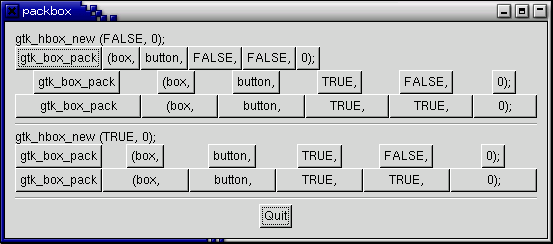
\includegraphics[height=50mm]{images/packbox1.png}
\caption{Méretarányos és homogén elhelyezésének a konténeren belül\cite{gtktut}}
\end{center}
\end{figure}

Ahogy korábban a kódsorokat, most a \textit{widget}ek sorait vesszük sorra a minél jobb megértés kedvéért.

\paragraph{Méretarányos elhelyezkedés}

\begin{description}
 \item[\texttt{expand} = \texttt{FALSE}, \texttt{fill} = \texttt{FALSE}] A konténerben lévő elemek -- ahogy fentiekben fogalmaztunk -- nem akarnak egymás rovására helyet szerezni (\texttt{epxand}), így a rendelkezésre álló vízszintes helyet nem is töltik ki, vagyis ezzel a megoldással az egész elemsorra nézve a szélekre történő igazítást (\texttt{pack\_start} esetén balra zárt, míg \texttt{pack\_end} esetén jobbra zárt) alakítható ki.

\index{konténer!size allocation@\textit{size allocation}}
 \item[\texttt{expand} = \texttt{TRUE}, \texttt{fill} = \texttt{FALSE}] Az összkép, leginkább az alatta található sor miatt kissé csalóka, mivel az elemek kissé rendezetlennek tűnnek, ehelyett viszont arról van szó, hogy minden egyes elem megszerezte magának -- a saját minimális méretigényének arányában -- az \texttt{expand} paraméter okán rendelkezésre álló plusz helyet és az így allokált (\textit{size allocation}) térrészen belül középen helyezkedik el.

 \item[\texttt{expand} = \texttt{TRUE}, \texttt{fill} = \texttt{TRUE}] Az egyes elemek nem csak hogy kiterjeszkednek (\texttt{expand}), hanem a korábban fel nem használt területre, de ki is töltik (\texttt{fill}) azt, azaz annak teljes méretében rajzolják is ki magukat. Ezzel a megoldással az elemsorra igaz, hogy az elemek között -- a konténer \texttt{spacing}, illetve a konténerbe helyezéskori \texttt{padding} paraméter értékével meghatározottaktól eltekintve -- térköz nincs.
\end{description}

Ahogy az az ábrából -- és talán a magyarázatból is -- kitűnik az \texttt{fill} opció állításának semmi teteje anélkül, hogy az \texttt{expand} be ne lenne kapcsolva, hisz e nélkül nincs semmilyen plusz terült, amire a \textit{widget} magát megnagyobbítva rajzolhatná.

\paragraph{Homogén elhelyezkedés}
\index{GtkBox@\texttt{GtkBox}!tulajdonságok!homogeneous@\texttt{homogeneous}}
\index{GtkBox@\texttt{GtkBox}!gyerek tulajdonságok!fill@\texttt{fill}}
\index{GtkBox@\texttt{GtkBox}!gyerek tulajdonságok!expand@\texttt{expand}}

\begin{description}
 \item[\texttt{expand} = \texttt{TRUE}, \texttt{fill} = \texttt{FALSE}] A konténerben lévő elemek -- a már használt kifejezéssel élve -- hiába akarnak egymás rovására helyet szerezni (\texttt{epxand}) a konténerben, a konténer a rendelkezésre álló vízszintes helyet egyenlően osztja el közöttük. Ezzel a megoldással az egész elemsorra igaz, hogy az elemek azonos helyet foglalnak el, de ezen helyen belül csak a minimálisan szükséges területre rajzolják ki magukat.

\index{konténer!size allocation@\textit{size allocation}}
 \item[\texttt{expand} = \texttt{TRUE}, \texttt{fill} = \texttt{TRUE}] A fentiekhez képest az eltérés csupán annyi, hogy az egyes elemek ki is használják -- ha úgy tetszik kitöltik (\texttt{fill}) az egyenlően kiporciózott térrészt, maximális méretben rajzolva ki magukat. A különbség az előző sorhoz képes épp az, mint a nem homogén konténerek esetén ugyanazon paraméterezés esetén.
\end{description}

\subsubsection{\texttt{GtkGrid}}
\index{GtkGrid@\texttt{GtkGrid}!tulajdonságok!row-homogeneous@\texttt{row-homogeneous}}
\index{GtkGrid@\texttt{GtkGrid}!tulajdonságok!column-homogeneous@\texttt{column-homogeneous}}

A \texttt{GtkGrid} típus szempontjából ugyanaz a két saját tulajdonság (\texttt{homogeneous}, \texttt{spacing}) számottevő, mint az imént \texttt{GtkBox} típus esetén amiket a fentiekhez hasonlóan befolyásol másik két paraméter. Ezek a paraméterek viszont ugyanúgy a konténer és a \textit{widget} viszonyát határozzák meg, mint az \texttt{expand} és a \texttt{fill} és azokhoz hasonló módon is működnek, ugyanakkor a \texttt{GtkWidget} tulajdonságai, tehát ott is tárolódnak.

\paragraph{Kiterjedés}

Az \texttt{expand} önálló tulajdonságként is létezik és szerepe gyakorlatilag ugyanaz, mint a \texttt{GtkBox} típus esetén, ugyanakkor mégis van egy számottevő különbség. Az \texttt{expand} voltaképpen másik két tulajdonság (\texttt{hexpand}, \texttt{vexpand}) -- amik a vízszintes és a függőleges kiterjedés szabályozzák --, együttes kezelésére szolgál, amik külön-külön is létező és értelmezett tulajdonságai a \textit{widget}nek.

\paragraph{Igazítás}

A \texttt{fill} gyerek-tulajdonság ebben a formában nem létezik, mint a \texttt{GtkWidget} típus tulajdonsága, viszont helyette két tágabban értelmezett tulajdonságot is használhatunk. Ez a tulajdonság az igazítás (\textit{align}), amit szintén megadhatunk külön vízszintes és függőleges (\texttt{halign}, \texttt{valign}) értelmezésben. A tulajdonság négy értéket vehet fel, amik közül egy a \texttt{FILL}, ami megegyezik a korábban részletezett \texttt{fill} gyerek-tulajdonság működésével. A mássága, illetve rugalmassága abban áll, hogy a másik három érték (\texttt{START}, \texttt{END}, \texttt{CENTER}) révén nem csak azt érhetjük el, hogy a \textit{widget} a rendelkezésre álló, felesleges vagy éppen szándékoltan megszerzett (\texttt{expand}) helyet kitöltse, hanem azt is, hogy annak elején, végén, vagy éppen közepén helyezze el magát. A pozíció természetesen függ az orientációtól, így a \texttt{START} érték jelenthet bal oldalt, vagy éppen felső pozíciót, ahogy az \texttt{END} jobb oldalt, vagy az üres térrész alját.

\subsection{Térköz, pányvázás és szegély}

\subsubsection{Fogalmak}

\paragraph{Térköz}
\index{GtkBox@\texttt{GtkBox}!tulajdonságok!spacing@\texttt{spacing}}
\index{GtkGrid@\texttt{GtkGrid}!tulajdonságok!row-spacing@\texttt{row-spacing}}
\index{GtkGrid@\texttt{GtkGrid}!tulajdonságok!column-spacing@\texttt{column-spacing}}

A konténer tulajdonsága, ami az benne elhelyezett elemek egymástól vett távolságát, vagyis ez egyes elemek közötti térközt határozza meg. Fontos megjegyezni, hogy a konténer első eleme előtt és utolsó elem után ez a térköz nem jelenik meg, csakis az elemek között. Ennek megfelelően az egy elemű konténerek ezen tulajdonsággal nem is rendelkeznek.

\paragraph{Pányvázás és szegély}
\index{GtkBox@\texttt{GtkBox}!gyerek tulajdonságok!padding@\texttt{padding}}

Ha a konténerben az egyes elemek között nem egyenlő térközt szeretnénk megadni, akkor lehetőség van az egyes \textit{widget}ek esetén külön-külön, csak az adott \textit{widget}re vonatkozó, a \textit{widget}et körülvevő térközt megadni. Ez a fajta térköz minden esetben megjelenik a \textit{widget} megfelelő oldalán és a már említett térközhöz hasonlóan szintén függ az orientációtól.

A \texttt{GtkBox} típus esetén csak egy -- az orientációtól függő irányban értelmezett -- térköz megadására van lehetőség, amit pányvázásnak (\textit{padding}) nevezünk és a \textit{widget} mindkét oldalán megjelenik. A \texttt{GtkGrid} típus ettől eltérően lehetőséget ad az oldalankénti (\textit{top}, \textit{bottom}, \textit{left}, \textit{right}) szegélyérték (\texttt{margin}) megadásra külön-külön, de kezelhetjük az összes oldal egyben is.

\subsubsection{\texttt{GtkBox}}

\vspace{12 pt}
\begin{figure}[H]
\begin{center}
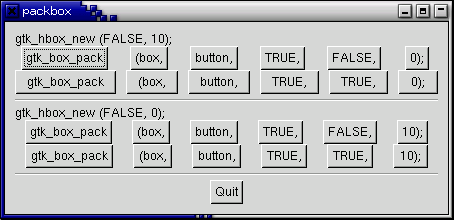
\includegraphics[height=50mm]{images/packbox2.png}
\caption{Tér az elemek között és körül a konténerben\cite{gtktut}}
\end{center}
\end{figure}

\paragraph{Tér az elemek között}
\index{GtkBox@\texttt{GtkBox}!tulajdonságok!spacing@\texttt{spacing}}

\begin{description}
 \item[\texttt{expand} = \texttt{TRUE}, \texttt{fill} = \texttt{FALSE}] Ez a példa nem mutatja meg igazán jól azt, hogy az elemek között jelenik meg az a térköz, amit a konténer létrehozásakor megadtunk, hiszen elemek nem töltik ki (\texttt{fill}) maximálisan a számukra rendelkezésre álló teret.
 \item[\texttt{expand} = \texttt{TRUE}, \texttt{fill} = \texttt{TRUE}] Mivel itt mindkét érték \texttt{TRUE}, a \textit{widget}ek a rendelkezésre álló teret teljes egészében kihasználják maguk megrajzolására, eltekintve természetesen a közöttük megjelenő 10 pixelnyi térköztől (\texttt{spacing}). Érdemes külön figyelmet fordítani a két szélső elemre, azoknak is az ablak széléhez közelebb eső részére a következő megoldással való összehasonlításhoz.
\end{description}

\paragraph{Tér az elemek körül}
\index{GtkBox@\texttt{GtkBox}!gyerek tulajdonságok!padding@\texttt{padding}}

\begin{description}
 \item[\texttt{expand} = \texttt{TRUE}, \texttt{fill} = \texttt{FALSE}] A \texttt{padding} megadásával a térköz nem az elemek között, hanem azok körül jelenik meg. Ez azt jelenti, hogy minden elem jobb és bal oldalán (függőleges elrendezés esetén felül és alul) egyaránt jelentkezik a megadott térköz, ennek okán közöttük annak -- függően a \texttt{fill} értékétől -- a kétszerese.

 \item[\texttt{expand} = \texttt{TRUE}, \texttt{fill} = \texttt{TRUE}] Ez az az eset amikor igazán jól látható a \textit{widget}ek között és az azok mellett megjelenő térköz 2:1 aránya. Az előbb -- a szélső widgetek elhelyezkedésénél megfigyelteket -- most hasznosíthatjuk, ha észrevesszük itt a szélső \textit{widget}ek nem tudnak a konténer széléig kiterjeszkedni, lévén két oldalról ki vannak párnázva (\texttt{padding}) 10-10 pixellel.
\end{description}

\subsubsection{\texttt{GtkGrid}}

Az imént leírtak a \texttt{GtkGrid}, illetve a \texttt{GtkWidget} típus saját tulajdonságainak használatával annyiban változnak, hogy a pányvázás (\texttt{padding}) helyett, szegélyezést alkalmazhatunk, vagyis minden oldal esetében külön-külön is megadhatjuk a \texttt{widget}et körülvevő térközt (\texttt{margin-top}, \texttt{margin-bottom}, \texttt{margin-left}, \texttt{margin-right}), amiket szintén kezelhetünk együtt (\texttt{margin}), ami íráskor az összes értéket felülírja, míg olvasáskor a legnagyobb értéket adja vissza. 

\section{A kód}

A fenti példaprogramok forrása a \href{http://developer.gnome.org/gtk-tutorial/stable/x386.html}{\textit{GTK+}} oldalán érhetők el.

\subsection{Fordítás és linkelés}

A korábbiakhoz hasonlóan az alábbi parancssor segítségével fordítható a példaprogram:

\lstccompile{gtk_packbox.c}{gtk_packbox}

\subsection{Futtatás}

Próbáljuk ezúttal a \texttt{./gtk\_packbox 1|2|3} paranccsal abban a könyvtárban, ahol a fordítást elkövettük, ahol a paraméter a teszt sorszáma, abban a sorrendben, ahogy azokat itt is ismertettük (a 3. természetesen csak ráadás).

\subsection{Eredmény}

Ha netán úgy érezzük mégsem világos mi is történik, mikor és miért a konténerekbe pakolás kapcsán, ne adjuk fel. Elsőre talán az egész mechanizmus jelentősége sem szembetűnő, ugyanakkor érdemes próbálkozni, azaz venni a forrást és játszani a különböző értékekkel (\textit{fill}, \textit{expand}, \textit{spacing}, \textit{padding}), illetve a létrehozott ablak átméretezésével.

\section{Tesztelés}

Amint azt már megállapítottuk, a konténerek segítségével alakíthatjuk ki a felhasználói felület szerkezetét. Ezen eszközök teszik lehetővé, hogy a \textit{widget}eket egymásba ágyazzunk, ezek határozzák meg a \textit{widget}ek konténerekben való elhelyezkedését, más \textit{widget}ekhez való viszonyát. Az így létrejövő szülő-gyerek viszonyok fa hierarchiát határoznak meg, aminek gyökerében maga az applikáció áll, második szintjén az applikáció egyes ablakai, ezek alatt pedig az ablakokon belüli \textit{widget}ek, a felületi elrendezésnek megfelelően.

A konténerek által kialakított szerkezet természetesen a tesztelés során is tetten érhető, bár nem szabad megfeledkeznünk arról, hogy a felhasználói felület tesztelésének alapjául szolgáló -- a szoftverek akadálymentesítéséhez (\textit{accessibility}) megalkotott -- réteg némiképp másként tekint a \textit{widget}ekre és a \textit{widget}ek közötti összefüggésekre, mint azt a \textit{GTK} teszi. Utóbbi természetesen erősen szoftverfejlesztői szemszöget képviseli, míg az előbbi a felhasználói gondolatvilágból indul ki, a felhasználók által értelmezett fogalmakból, szerkezetből, összefüggésekből, tulajdonságokból építkezik, ebből adódnak azok az eltérések, amiket a későbbikben folyamatosan számba veszünk.

\subsection{Gyerekek keresése}

Az előző részben említett \texttt{GenericPredicate} nem csak szűrt keresések lebonyolítására alkalmas. Az alapértelmezett paraméterekkel létrehozott objektum használatának eredménye a gyakorlatban pont az, hogy az így létrejött elvárásoknak minden elem megfelel. Egy adott \texttt{Node} \texttt{findChild} függvénynek átadva az előbbi módszerrel létrehozott \textit{predicate} objektumot, annak gyerekeit kaphatjuk vissza. Amennyiben a \texttt{findChild} függvény \texttt{recursive} paramétere \texttt{True}, akkor az összeg gyereket, amennyiben \texttt{False}, akkor csak a közvetlen gyerekeket.

Azt már elöljáróban is érdemes megjegyezni, hogy a \textit{GTK} \textit{widget}ek által létrehozott hierarchia, illetve az \textit{accessibility} eszközök által lekérdezhető elemek hierarchiája nem egyezik meg tökéletesen. Bizonyos elemek esetén eltérések lehetnek, amiket azt adott helyen részletezünk.
